%% SingularityNET Marketplace Assistant Design Document
%%
%% Render with:
%% ./render.sh

\documentclass[]{article}
\usepackage{url}
\usepackage{minted}
\usepackage[hyperindex,breaklinks]{hyperref}
\usepackage{breakurl}
\usepackage{listings}
\lstset{basicstyle=\ttfamily\footnotesize,breaklines=false,frame=single}
\usepackage{float}
\restylefloat{table}
\usepackage{longtable}
\usepackage{graphicx}
\usepackage[font=small,labelfont=bf]{caption}
\usepackage[skip=0pt]{subcaption}
\usepackage{circledsteps}

\begin{document}

\title{SingularityNET Marketplace Assistant Design Document\\
  \texttt{(DRAFT)}} \author{Nil Geisweiller}
\maketitle

\section{Introduction}
After the explosion of popularity and capability of LLMs, it was
decided to reorient the AI-DSL project to incorporate these tools at
the earliest stage.  The purpose of this document is to lay out a
provisional design for such integration.  The long-term goals of the
AI-DSL project, mainly to use formal verification for composing AI
services, remain unchanged, but what have changed are the priorities.
Given the state of advancement of LLMs it seems now possible to offer
natural language as the main, and earliest, user interface of the
AI-DSL.  For this reason it was rebranded as the SingularityNET
Marketplace Assistant, as spontaneously suggested by Alexey Potapov
during a meeting.

In addition to being used for the user interface, LLMs can also take
over some tasks that would otherwise have been carried out by
specialized programs, such as synthesizing AI service compositions.
Traditionally, in order to do that well, it would require to provide
more descriptive formal specifications of AI services.  However, by
taking into consideration natural language descriptions, that are
already available to any AI service on the marketplace, LLMs can
potentially suggest compositions taking semantics into account.  An
example of that is HuggingGPT~\cite{Shen2023}.  Given the brittleness
of LLMs, it is expected that they will not replace advanced formal
methods.  However, it is also expected that by combining LLMs'
semantic capabilities with weaker-than-initially-envisioned but
already accessible formal methods, moderately useful and reliable AI
service compositions can be achieved.  Every AI service on the
Marketplace has a Protocol Buffers (protobuf) specification.  Early
experiments suggest that formally verifying compositions of AI
services based on their protobuf specifications is also
doable~\cite{ProtobufCheckingXP2023}.

\section{Generic Interaction}
Before presenting to the design of the SingularityNET Marketplace
Assistant, or \emph{SMA} for short, let us start by describing a
generic user interaction to give an idea of the functionality we want
to accomplish.
\begin{enumerate}
\item A natural language query comes into the SMA.
\item
  \begin{enumerate}
  \item The SMA processes the query and returns a suggestion of AI
    service composition, formulated in natural, formal and graphical
    languages.
  \item Ideally, information pertaining to cost, expected performance
    and time estimate of completion is provided as well.
  \end{enumerate}
\item
  \begin{enumerate}
  \item Either the user confirms and triggers the execution of the
    composition,
  \item or
    \begin{enumerate}
    \item either provides feedback to repeat the process from step 2,
    \item or abort.
    \end{enumerate}
  \end{enumerate}
\item The SMA returns the result of the query, its content alongside a
  description of it.
\item The user may optionally provide some final feedback, possibly
  repeating the process from step 1, 2 or 3.
\end{enumerate}
All interactions happen in natural language, possibly complemented
with other media when appropriate.

\section{Provisional Design}
No precise commitments have yet been made to achieve such
functionality.  Some provisional design, subject to change, is
nonetheless provided below.
\begin{itemize}
\item \textbf{Step 2} of the generic interaction described above could
  be achieved by having an LLM, pre-tuned, pre-prompted or otherwise,
  that knows:
  \begin{enumerate}
  \item The goals to achieve (find and compose services to fulfill the
    user's query).
  \item The marketplace (formal and informal descriptions of all AI
    services on the SingularityNET Marketplace).
  \item The format in which to return the suggested composition.
  \end{enumerate}
  Subsequently to processing the user's query, the LLM would output a
  composition, in the accepted format decided above, to be formally
  checked based on the protobuf specifications of the AI services
  involved.  Such format remains to be determined, it could be Python,
  SUO-KIF, MeTTa or otherwise.  The precise mechanism for checking
  remains to be determined as well.  Early experiments indicate that a
  Python type checker such as mypy can be used when the protobuf
  compilation generates type annotated Python
  code~\cite{ProtobufCheckingXP2023}.  The checking step could be
  visible or invisible to the user, that also remains to be
  determined.
  \begin{itemize}
  \item If the checking is successful, then the SMA would instruct the
    LLM to output such composition to the user, in natural, formal and
    graphical languages.  How to obtain the cost, performance
    evaluation and time estimate of running the composition remains to
    be determined.  It was originally suggested to use an existing
    Dependently Typed Language like Idris~\cite{AIDSLReport2021}.  In
    the light of both LLMs and Hyperon/MeTTa developments, this needs
    to be re-evaluated.
  \item If the checking is unsuccessful, then the SMA would provide
    feedback to the LLM, requesting another suggestion of composition,
    and so on.  Whether this back and forth between the LLM and SMA
    should be visible or invisible to the user remains to be
    determined.
  \end{itemize}
\item \textbf{Step 3} is handled by the LLM again, which expects from
  the user an acceptation or a rejection of the suggestion, plus
  possibly some feedback on how to improve it.  The workflow, whether
  to repeat the process from step 2, abort, or prepare to trigger a
  transaction, would be decided by the LLM.  If the LLM infers that
  the user agrees to run the composition, then a final confirmation
  step would be presented to the user, and if confirmed then handed to
  the blockchain management software of SingularityNET (which,
  depending on how it is set-up, may result in more confirmation
  steps).  Precisely how the composition would be run remains to be
  determined.  It could be handled by a dedicated composition-service
  on the SingularityNET Marketplace, so once that service has received
  enough fund to cover the cost of all AI services of the composition,
  it can run the whole thing in isolation.  Other scenarios are
  possible as well.  For instance the user's client machine could do
  the dispatching.  This would however require more involvement and
  confirmation steps from the user.  Ideally, multiple ways could be
  offered which the user may choose from.  In general, we should also
  be opened to the fact that since everything is open source, the
  whole process, from composition to execution could be run locally
  and not involve any transaction on the SingularityNET platform,
  though this would likely be left to the tinkerers only.
\item In \textbf{Step 4}, the LLM would receive the output of the AI.
  It may attempt to add a natural language description to complement
  its output.  This could be as simple as confirming that the output
  is in the desired format, if for instance it is too difficult to
  read its content, a video or such, or maybe the user expressed the
  desire to not read the content.
\item In \textbf{Step 5}, the LLM would process the final user
  feedback, if any.  What do to with that information remains to be
  precisely determined.  If the LLM infers that the user is satisfied,
  then it may stop there with a greeting message.  Otherwise, if the
  user is not satisfied and some useful feedback has been provided,
  then the LLM may offer to re-start from a previous step.
\end{itemize}

\section{Project Planning}
A detailed plan still needs to written.  I believe the objective would
be to have something close to what has been described above within 4
to 6 months [correct me if I'm wrong, Matt].  Of course it is to be
expected that some problems may turn out to be more difficult than
anticipated.  But as such plan is put together, a few milestones
already providing value could be set.  For instance, initially the LLM
goals could be reduced to retrieving a single service that closely
matches the user's query, leaving composition and even execution
aside.  Or, and that can occur in parallel, a composition-service can
be implemented, etc.

Another thing to keep in mind is the longer-term planning.  Past this
4 to 6 months time frame we want to progressively incorporate more and
more formal methods into the process to increase reliability and
performance.  The short-term planning should take that into account.

\section{Examples}
This section goes over examples of User$\leftrightarrow$SMA
interactions.  It is more or less a recycling of that previous
document~\cite{Assemblage2022}.  Note that nearly all AI services
involved in these examples already exist on the SingularityNET
Marketplace.

\subsection{Recognize Emotion of Hand Written Text}
\begin{enumerate}
\item \textbf{User}: ``I have a dozen handwritten letters scanned in
  that document.  Could you read it and tell me if the overall
  sentiment is positive or negative?''
\item \textbf{SMA}: ``Sure, I found that by composing the two services
  below I should be able to do that.  This will cost you 0.2 AGIX,
  should take half a second, and is expected to give you the correct
  answer with a probability of 0.75.  I have included a logical and
  graphical representation of that composition below.  Do you want me
  to proceed?''
  \begin{minted}[mathescape]{scheme}
    (. emotionRecognition handWritingToText)
  \end{minted}
  \begin{figure}[H]
    \centering
    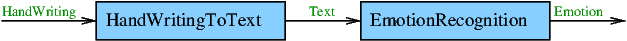
\includegraphics[scale=0.45]{figs/HandWritingEmotionRecognition.png}
  \end{figure}
\item \textbf{User}: ``0.75 probability... OK, do it anyway''
\item \textbf{SMA}: ``Here's the result: the overall sentiment is
  positive.  You may find additional information below, including the
  intermediary result of each service.''\\
  $\dots$
\item \textbf{User}: ``Thank you, I'm 75\% relieved''
\item \textbf{SMA}: ``You're welcome, can I do anything else?''
\item \textbf{User}: ``No, I'm good for now''
\end{enumerate}

\subsection{Topic Analysis of Speech}
\begin{enumerate}
\item \textbf{User}: ``Oh no!  My boss wants me to go through these
  meeting recordings from the past 5 years and label them by topic.
  All that by the end of today.  Please help me!''
\item \textbf{SMA}: ``Don't panic, I should be able to do that by
  composing the two services below and iterating over all recordings.
  This will cost you 8 AGIX overall, should take 12 seconds, and is
  expected to give you the correct label on each recording with a
  probability of 0.92.  I have included a logical and graphical
  representation of that composition below.  Do you want me to
  proceed?''
  \begin{minted}[mathescape]{scheme}
    (map (. topicAnalysis speechToText))
  \end{minted}
  \begin{figure}[H]
    \centering
    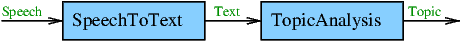
\includegraphics[scale=0.55]{figs/SpeechTopicAnalysis.png}
  \end{figure}
\item \textbf{User}: ``Oh good lord, proceed immediately!''
\item \textbf{SMA}: ``Here's the results.  I've synthesized them in a
  table mapping each file name to its topic.''\\
  $\dots$
\item \textbf{User}: ``You rock!''
\item \textbf{SMA}: ``Thanks for your compliment, can I do anything
  else?''
\item \textbf{User}: ``No, that was already a lot''
\end{enumerate}

\subsection{Turn an English Song into a Chinese Song}
\begin{enumerate}
\item \textbf{User}: ``I found this old song in my collective work.  I
  like the instrumental part, but the singing is a bit lame.  I was
  thinking of replacing it by something more interesting, say some
  Chinese female singing.  Unfortunately I no longer have the
  multi-track recording, only that stereo audio file.  Do you think
  you could do the exploit of replacing the singing, leaving the
  instrumental part untouched?  Oh, and BTW the lyrics matter, you
  need to keep those, just translate them in Chinese instead.  Can you
  do it?''
\item \textbf{SMA}: ``Turns out I can, by composing these 6 services
  below.  It will cost you 12 AGIX, should take 28 seconds, and is
  expected to give you at least a moderate level of satisfaction with
  a probability of 0.69.  I have included a logical and graphical
  representation of that composition below.  Do you want me to
  proceed?''
  \begin{minted}[mathescape]{scheme}
    (lambda x (let (enSing accomp)
                   (Spleeter x)
                   (let* ((enLyrics (toText enSing))
                          (chLyrics (toChinese enLyrics))
                          (notes (toMidi enSing))
                          (chSing (chineseSing notes chLyrics)))
                          (Mixer accomp chSing))))
  \end{minted}
  \begin{figure}[H]
    \centering
    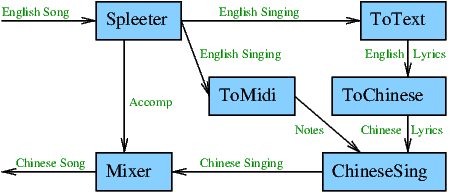
\includegraphics[scale=0.55]{figs/EnglishToChineseSong.png}
  \end{figure}
\item \textbf{User}: ``Wow, I'm impressed, yeah you can proceed''
\item \textbf{SMA}: ``Here's the final result, as well as all
  intermediary results from all services.  Hope you like it.''\\
  $\dots$
\item \textbf{User}: ``Wait, the timing is completely off!  She is not
  singing when she should.  Can you fix that?''
\item \textbf{SMA}: ``I am sorry to hear that.  I don't know if I will
  be able to fix it, if not you can also try to resync the Chinese
  singing yourself by combining the output of the ChineseSing service
  with the instrumental output of the Spleeter service.''
\item \textbf{User}: ``I see.  Well, I'll try to do the last bit
  myself then.  That was already helpful.''
\end{enumerate}

\section{conclusion}
TODO

\bibliographystyle{splncs04}
\bibliography{local}

\end{document}
